\section{A competitive RNN against the transformer}
The best RNN of the whole study is compared with the baseline transformer here on the same probes (the P4 section reports which RNN that is; this section uses the supplied modern tanh RNN at $\lr=0.002$ and the d8 baseline at $0.003$ because both have every probe, and the P4 figures show the same statistics for the GRU family). Figure~\ref{fig:cmp} plots the activation RMS of the residual stream at every position and the cosine between stream states at different positions, per depth index.

\paragraph{Across layers.} Both models grow their stream with depth and change its direction mostly in the first two branches (Figures~\ref{fig:p1stages} and~\ref{fig:p2stages}), but the scales are very different: the transformer stream ends at RMS 24 and the RNN stream at 1.7, because the RNN's recurrent branches pass through a tanh and its MLP outputs stay near the stream scale, while the transformer's first attention and MLP branches emit outputs 6 to 20 times their input. The transformer's full loss gradient decays by 50 from embedding to final stream and the RNN's by 10, so the RNN's depth is, if anything, better conditioned; its problem is time, not depth.

\paragraph{Across positions.} The transformer has one special position. At $t=0$ its final stream RMS is 90, four times the 22 to 25 at every other position, which is the massive activation that every head attends to as a sink (Section 2.3). The RNN has the opposite special position: its state at $t=0$ is small (RMS 0.5 against 1.6 to 1.8 later) because the recurrence starts from zero and needs a few steps to reach its working range. Away from $t=0$ the RMS of both models is flat in position. The cosine between stream states one position apart rises from 0.05 at the embedding to 0.45 to 0.5 in the transformer's middle and upper layers and stays near that value for lag 64 and for the cosine to the first position (0.25 to 0.35): the transformer keeps a shared, position independent component (the sink direction and a mean token direction) plus a token specific part. The RNN's lower layers have almost orthogonal states at adjacent positions (cosine 0.1 for layers 1 and 2) and its upper layers reach 0.48, similar to the transformer, but their similarity falls off faster with lag (0.36 at lag 64, 0.34 to the first position). Measured on the hidden states themselves rather than the stream, the RNN's upper layers are far smoother in time (cosine 0.93 at lag 64 in layer 4, Section 3.2), so the recurrent branches carry a slow state and the stream adds a fast, token specific component through the MLPs. The gated residual variants of both families have lower cross position similarity at every depth (transformer 0.2 to 0.3 at lag 64, RNN 0.02 to 0.15), that is, the gates remove some of the shared component.

\paragraph{Context.} The practical difference is in Table~\ref{tab:p2ctx} and Figure~\ref{fig:p1ctx}: the transformer still improves from tokens 256 to 1023 and loses 1.7 nats when cut to 16 tokens, whereas the RNN gains nothing measurable beyond 64 tokens and its last token gradient underflows within 90 steps. The transformer's 0.4 nat advantage in full loss (2.83 against 3.33 on the probe sequences) is the long context it can use and the RNN cannot.

\begin{figure}[h]\centering
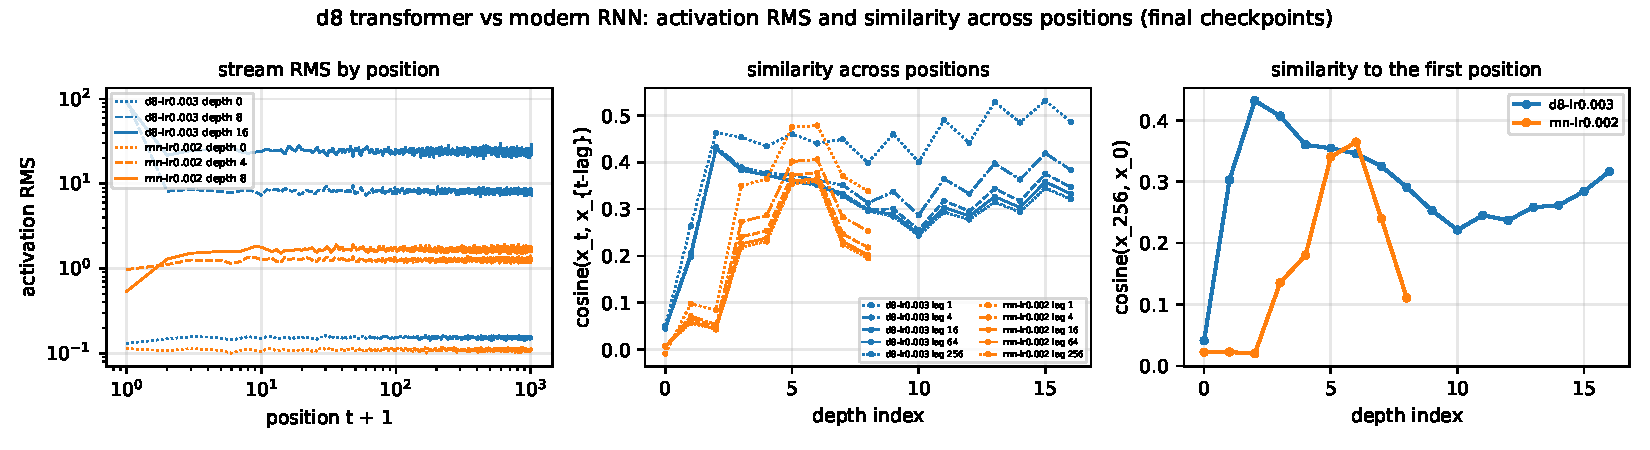
\includegraphics[width=\linewidth]{cmp_positions.pdf}
\caption{Transformer d8 against the modern RNN. Left: stream RMS at every position for the embedding, the middle branch input and the final stream. Middle: cosine between stream states at lags 1 to 256 against depth. Right: cosine between position 256 and position 0.}
\label{fig:cmp}
\end{figure}
